\documentclass{standalone}
\usepackage{tikz}
\usetikzlibrary{hobby}
\usetikzlibrary{patterns}

\usepackage{fkmath}
\begin{document}
  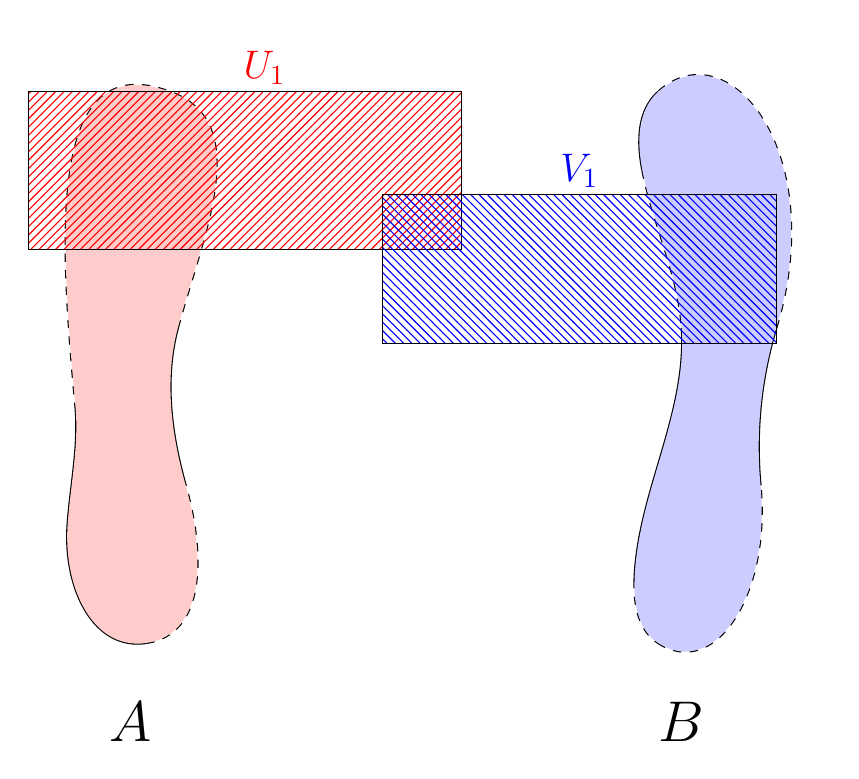
\begin{tikzpicture}[use Hobby shortcut]
    %% Blob
    \begin{scope}
      \draw[thick, closed=true] (0,-1) .. ([blank=soft].5,1) .. (.4,3) .. ([blank=soft].3,6) .. ([blank=soft]-.9,2) .. (-1,.5);
      \draw[dashed, thick, use previous Hobby path={invert soft blanks, disjoint}];
      \fill[red!20!white, closed=true] (0,-1) .. (.5,1) .. (.4,3) .. (.3,6) .. (-.9,2) .. (-1,.5);
      \node (A) at (-.2,-2) {\huge $A$};
    \end{scope}

    \begin{scope}
      \draw[thick, closed=true] ([blank=soft]6.5,-1) .. ([blank=soft]7.8,1) .. (8,3) .. ([blank=soft]6.5,6) .. (6.3,5) .. ([blank=soft]6.8,3) .. (6.2,-.2);
      \draw[dashed, thick, use previous Hobby path={invert soft blanks, disjoint}];
      \fill[blue!20!white, closed=true] (6.5,-1) .. (7.8,1) .. (8,3) .. (6.5,6) .. (6.3,5) .. (6.8,3) .. (6.2,-.2);
      \node (B) at (6.8,-2) {\huge $B$};
    \end{scope}

    % Help in positioning diagrams when modifying
    % \draw[help lines, color=gray!30, dashed] (-1.9,-2.9) grid (9.9,6.9);
    % \draw[->] (-2,0)--(10,0) node[right]{$x$};
    % \draw[->] (0,-3)--(0,7) node[above]{$y$};

    \draw[pattern=north east lines, pattern color=red] (-1.5,6) rectangle (4, 4);
    \draw[pattern=north west lines, pattern color=blue] (8,4.7) rectangle (3, 2.8);
    \node (U1) at (1.5,6.3) {\Large \color{red} $\ol{U_1}$};
    \node (U1) at (5.5,5) {\Large \color{blue} $\ol{V_1}$};
  \end{tikzpicture}
\end{document}